\documentclass{article}
% generated by Madoko, version 1.1.6
%mdk-data-line={1}


\usepackage[heading-base={2},section-num={False},bib-label={hide},fontspec={True}]{madoko2}
\usepackage{float}


\begin{document}



%mdk-data-line={7}
\mdxtitleblockstart{}
%mdk-data-line={7}
\mdxtitle{\mdline{7}Initial Experiments}%mdk
\mdxauthorstart{}
%mdk-data-line={12}
\mdxauthorname{\mdline{12}21 January 2019}%mdk
\mdxauthorend\mdtitleauthorrunning{}{}\mdxtitleblockend%mdk
\mdline{9}
\begin{mdtoc}%mdk

\section*{Contents}\label{sec-contents}%mdk%mdk

\begin{mdtocblock}%mdk

\mdtocitemx{sec-initial-experiments}{\mdref{sec-initial-experiments}{1.\hspace*{0.5em}Initial Experiments}}%mdk

\begin{mdtocblock}%mdk

\mdtocitemx{sec-calibrating-the-filters}{\mdref{sec-calibrating-the-filters}{1.1.\hspace*{0.5em}Calibrating the filters}}%mdk

\mdtocitemx{sec-calibrating-the-leds}{\mdref{sec-calibrating-the-leds}{1.2.\hspace*{0.5em}Calibrating the LEDs}}%mdk

\mdtocitemx{sec-set-up-distances}{\mdref{sec-set-up-distances}{1.3.\hspace*{0.5em}Set up distances}}%mdk

\mdtocitemx{sec-finding-relationship-between-the-sensor-output-and-lux}{\mdref{sec-finding-relationship-between-the-sensor-output-and-lux}{1.4.\hspace*{0.5em}Finding relationship between the sensor output and Lux}}%mdk

\mdtocitemx{sec-angles-to-test}{\mdref{sec-angles-to-test}{1.5.\hspace*{0.5em}Angles to test}}%mdk
%mdk
\end{mdtocblock}%mdk
%mdk
\end{mdtocblock}%mdk
%mdk
\end{mdtoc}%mdk

%mdk-data-line={11}
\section{\mdline{11}1.\hspace*{0.5em}\mdline{11}Initial Experiments}\label{sec-initial-experiments}%mdk%mdk

%mdk-data-line={13}
\subsection{\mdline{13}1.1.\hspace*{0.5em}\mdline{13}Calibrating the filters}\label{sec-calibrating-the-filters}%mdk%mdk

%mdk-data-line={15}
\begin{quote}%mdk

%mdk-data-line={15}
\noindent\mdline{15}Calibrate the polarising filters to establish a common \mdline{15}\textquotedblleft{}zero degrees\textquotedblright{}\mdline{15} angle (or datum)%mdk
%mdk
\end{quote}%mdk

%mdk-data-line={17}
\noindent\mdline{17}Each filter sheet arrived as a 10cmx10cm sheet, which was aligned vertically in packaging. The sheet was split into four 5cm5xcm segments, and the vertical was marked on each. The sheets were then cut, and each of the 8 squares was stuck to circular sheets of card with square cut outs. This means that angles could be marked on the perimeter, and the sheets can be rotated easily.%mdk

%mdk-data-line={19}
\mdline{19}The circular filters were then double checked for their \mdline{19}\textquotedblleft{}0 degrees\textquotedblright{}\mdline{19} mark by aligning each, and ensuring that all light passed through at 0 degrees, and all light was blocked at 90 degrees.%mdk

%mdk-data-line={21}
\subsection{\mdline{21}1.2.\hspace*{0.5em}\mdline{21}Calibrating the LEDs}\label{sec-calibrating-the-leds}%mdk%mdk

%mdk-data-line={23}
\begin{quote}%mdk

%mdk-data-line={23}
\noindent\mdline{23}Find a suitable voltage and brightness for the LEDs to optimise results, but maintain steady LED performance;%mdk
%mdk
\end{quote}%mdk

%mdk-data-line={25}
\noindent\mdline{25}The Microcontroller used for this investigation (Raspberry Pi Model 3A+) provides a regulated 3.3V output. This was connected to a 10mm white LED, which then provided sufficient intensity to be used in the experiment.%mdk

%mdk-data-line={27}
\subsection{\mdline{27}1.3.\hspace*{0.5em}\mdline{27}Set up distances}\label{sec-set-up-distances}%mdk%mdk

%mdk-data-line={29}
\begin{quote}%mdk

%mdk-data-line={29}
\noindent\mdline{29}Find a suitable distance for the equipment to maximize accuracy but allow room for the apparatus to be used;%mdk
%mdk
\end{quote}%mdk

%mdk-data-line={31}
\noindent\mdline{31}The equipment was set up with a clamp stand for each equipment, and the component were aligned so that the bases were as close as possible. This resulted in the components being close enough together so as to avoid significant reduction in intensity due to the inverse square law.%mdk

%mdk-data-line={34}
\subsection{\mdline{34}1.4.\hspace*{0.5em}\mdline{34}Finding relationship between the sensor output and Lux}\label{sec-finding-relationship-between-the-sensor-output-and-lux}%mdk%mdk

%mdk-data-line={35}
\begin{quote}%mdk

%mdk-data-line={35}
\noindent\mdline{35}Compare the raw output data of the sensor to a lux-meter to find a suitable range and sensitivity. This will also help me convert the arbitrary units of the sensor to Lux value%mdk
%mdk
\end{quote}%mdk

%mdk-data-line={37}
\noindent\mdline{37}Firstly, the equipment was set up as shown in the diagram: clamp stands holding each the LED, sensor, and polarising filters. A Luxmeter was then attached just above the sensor with another clamp stand, so that the spread of light was even on both the sensor and diagram (a sheet of paper was used to achieve this).%mdk

%mdk-data-line={39}
\mdline{39}Measurements were then taken comparing the output of the sensor to the readings on the Luxmeter. These were taken at suitable  intervals to produce a line of best fit. The results are shown below in\mdline{39}~\mdref{tab-sample}{\mdcaptionlabel{1}}\mdline{39}%mdk

%mdk-data-line={41}
\begin{table}[H]%mdk
\begin{mdcenter}%mdk
\begin{mdtabular}{2}{\dimeval{(\linewidth)/2}}{1ex}%mdk
\begin{tabular}{ll}\multicolumn{1}{c}{{\mdseries\mdline{42}Raw sensor output}}&{\mdseries\mdline{42} Luxmeter (Lux x10)}\\

\midrule
\mdline{44} 854&\mdline{44} 124\\
\mdline{45} 695&\mdline{45} 97\\
\mdline{46} 552&\mdline{46} 77\\
\mdline{47} 346&\mdline{47} 45\\
\mdline{48} 123&\mdline{48} 14\\
\mdline{49} 119&\mdline{49} 13\\
\mdline{50} 13&\mdline{50} 0\\
\midrule[\dimpx{2}]
\end{tabular}\end{mdtabular}

%mdk-data-line={53}
\mdhr{}%mdk

%mdk-data-line={54}
\noindent\mdline{54}\mdcaption{\textbf{Table~\mdcaptionlabel{1}.}~\mdcaptiontext{Initial experiment to find the relationship between sensor output and lux}}%mdk
%mdk
\end{mdcenter}\label{tab-sample}%mdk
%mdk
\end{table}%mdk

%mdk-data-line={55}
\mdline{55}These results were plotted on a scatter graph, and a line of best fit was generated:%mdk

%mdk-data-line={57}
\mdline{57}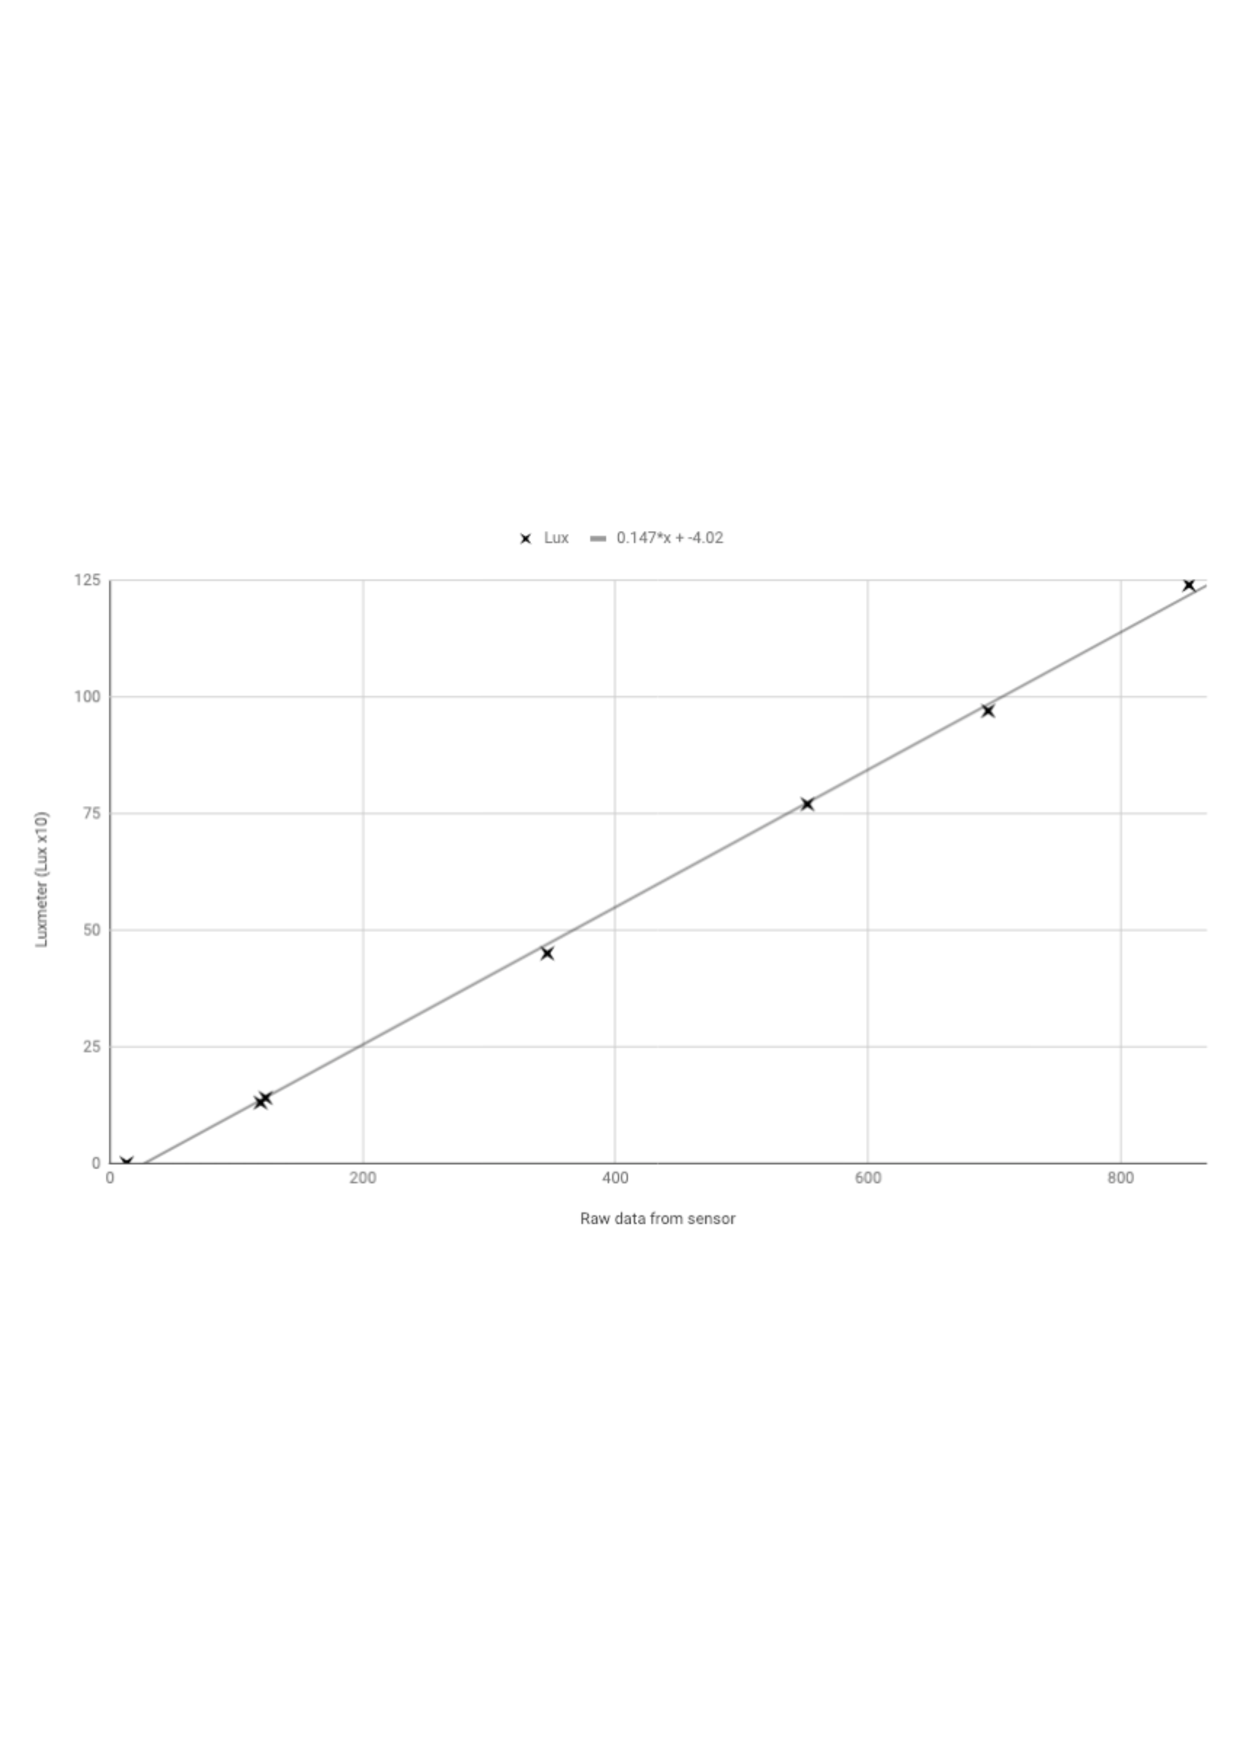
\includegraphics[keepaspectratio=true,width=\dimmin{}{\dimwidth{0.90}}]{images/results}{}\mdline{57}%mdk

%mdk-data-line={61}
\noindent\mdline{61}This means that the equation of line of best fit is \mdline{61}$y=0.147x-4.02$\mdline{61}, which means that \mdline{61}$\text{Lux}\approx\text{Raw data}*0.147$\mdline{61}%mdk

%mdk-data-line={63}
\subsection{\mdline{63}1.5.\hspace*{0.5em}\mdline{63}Angles to test}\label{sec-angles-to-test}%mdk%mdk

%mdk-data-line={65}
\begin{quote}%mdk

%mdk-data-line={65}
\noindent\mdline{65}Find suitable increments of angles to produce accurate results in a reasonable time scale.%mdk
%mdk
\end{quote}%mdk

%mdk-data-line={67}
\noindent\mdline{67}The radius of each circular filter is \mdline{67}\textasciitilde{}\mdline{67}7cm, which means that there is enough space on the perimeter to mark off each 5 degrees between 0 and 90 degrees. This means that a total of 18 intervals can be taken, which gives enough to form a reliable set of data.%mdk%mdk


\end{document}
